\documentclass[11pt]{article}                                                   
\usepackage[colorlinks]{hyperref}                                               
\usepackage{breakurl}                                                           
\usepackage{amsmath}                                                            
\usepackage[margin=.9in]{geometry}                                              
\newcommand{\nx}{\texttt{quigley}}                                              
\newcommand{\sechost}{\texttt{secureIpums}}                                     
\newcommand{\repo}{\texttt{/home/ipums-repo}}                                   
\newcommand{\ipums}{\texttt{$\sim$/IPUMS}}                                      
%\newcommand{\uP}{$\square$}                                                    
\newcommand{\ar}{$\rightarrow$}                                                 
\newcommand{\user}[1]{\texttt{#1}}                                              
\usepackage{mdframed}                                                           
%\usepackage{color}                                                             
%\usepackage{framed}                                                            
\usepackage{xcolor}       
\usepackage{graphicx}
\begin{document}

\title{The Rstudio175 cloud server\\
for Demog/Econ C175}

\maketitle
\tableofcontents

\section{Introduction}

The Rstudio175 cloud server is the computing infrastructure for all of the homework assignments in Demog/Econ 175. If you are not enrolled in this course, please hang up and dial 9-1-1.  \textbf{If you are a concurrent enrollement student, keep reading but also please send email to c175@demog.berkeley.edu}.

\begin{mdframed}[backgroundcolor=blue!20]        
\textbf{There are two ways to use Rstudio}. We recommend using the \textbf{Rstudio175 Cloud Server} described below. However it is also possible to  to install the \textbf{Desktop} version of  Rstudio on your own machine and run program locally.

The Rstudio175 Cloud Server, will be maintained and supported so as to optimize your experience in Demography/Economics C175 and minimize your need to be your own system administrator.  \textbf{There is no need to install Desktop Rstudio} unless you either like  being your own sys/admin ,or you plan to do your homework on a planet where there is no internet\footnote{Another good reason to install Desktop Rstudio is if you plan to use R for projects outside of Demog/Econ C175}. Be aware that you're pretty much on your own with the Desktop version.  
\end{mdframed}
\section{Logging in to the Rstudio175 Cloud Server for the first time}

Shortly after registering for C175, you should receive email with instructions on how to initialize your account by setting your password.  All you should need to do is click on the link included in the email, and provide a new password.  If you never received this email verify that you are registered, then send email to trouble@demog.berkeley.edu.  Note that you must initialize your account within two weeks of the start of the semester to avoid administrative hurdles.

Once you have established a password for your Rstudio175 Cloud account, go to 
\url{http:courses.demog.berkeley.edu/goldstein175}.  The top of the page looks like this:

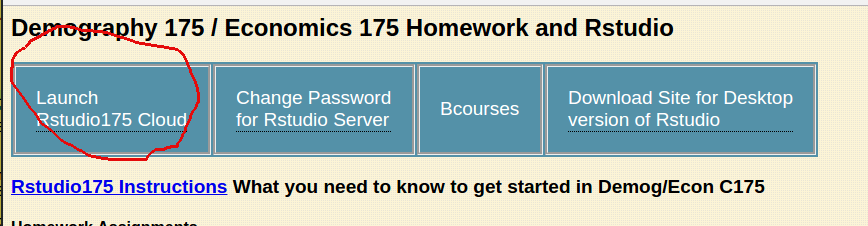
\includegraphics[scale=.5]{WebsiteTop}

Unsurprisingly, the button labeled ``Launch Rstudio175 Cloud'' will launch the Rstudio Cloud Server in a separate window or browser tab. 

\vspace{.5cm}

With any luck you should soon be confronted with a web page sporting the Rstudio login dialog:

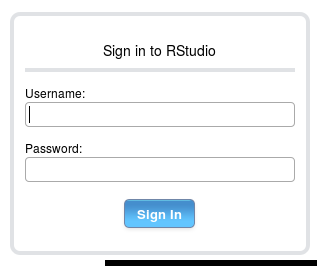
\includegraphics[scale=.35]{RstudioSignin}

Your username, (as indicated in the above mentioned email) is your
calnet ID (that is, the part of your @berkeley.edu email address that comes before the '@'. \textbf{but your password is whatever you set it to be}:
Rstudio175 uses an entirely separate password database from that of
Calnet.

\section{Some things to notice about Rstudio}

Once you have successfully given your Calnet ID and password, your browser window becomes a modern IDE\footnote{IDE stands for \emph{Integrated Development Environment} which means a computer program that helps you write computer programs.} IDEs are quite complicated programs used by professionals to make writing programs more efficient and less error prone.

You will use only a small fraction of the features of Rstudio -- but should you (wisely) go on to master R, you will come to be amazed at the cleverness of this thing. Unfortunately,  before amazement comes bewilderment at the number of features present.

Your initial Rstudio window should look something like this:

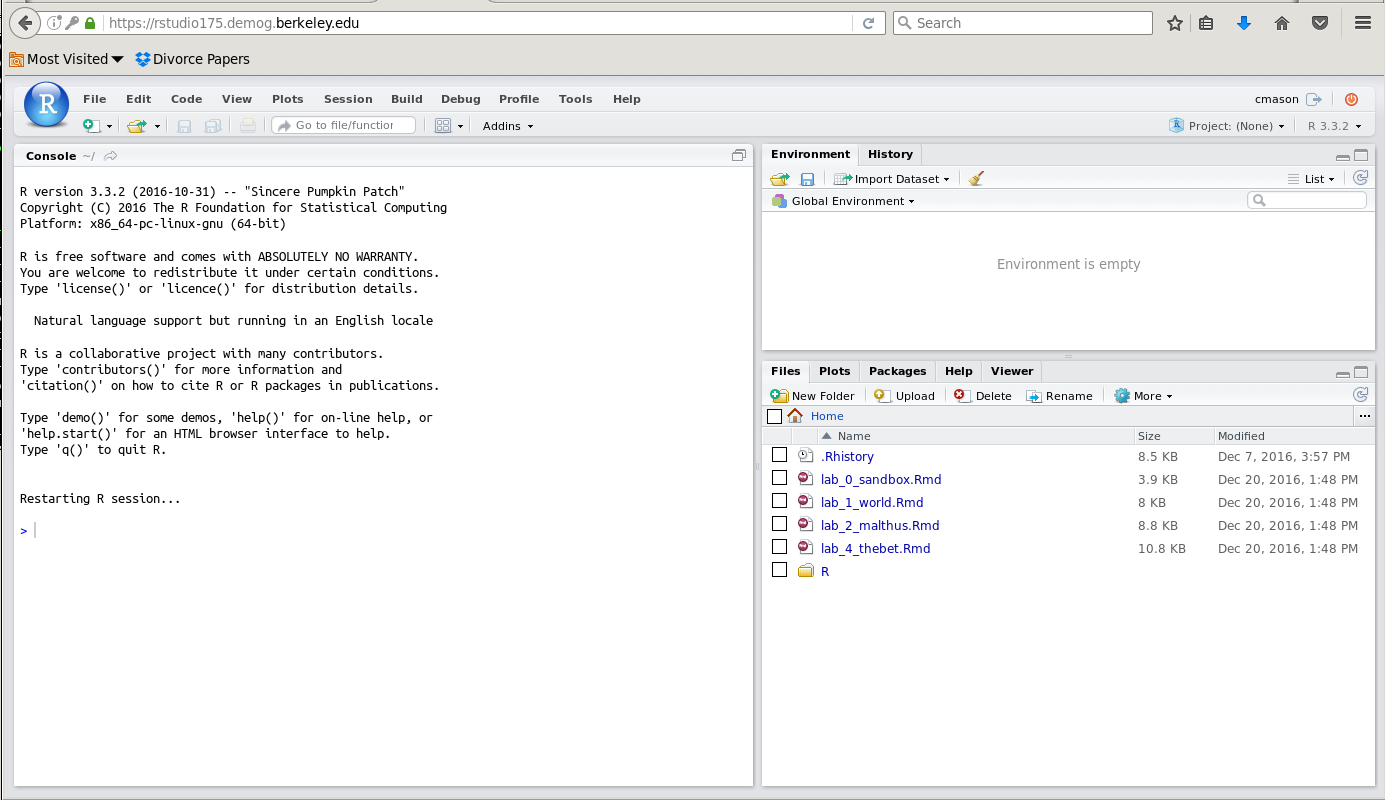
\includegraphics[scale=.35]{RstudioStart}

\textbf{BEFORE touching anything} Please Notice the following:

\begin{itemize}
\item The left hand pane, labeled ``console''  is an R interpreter.  It functions just like  \url{http://tryr.codeschool.com/}. It provides a prompt ``>'' at which you can type R commands and, unless assigned to a variable, it prints the result on a subsequent line.

\begin{verbatim}

> 1+1
[1] 2
> sqrt(152399025)
[1] 12345
> x<-1:999
> y<-log(x)
> plot(x,y)
\end{verbatim}



 \textbf{YOU HAVE been to tryr.codeschool.com right?} If not go there right now and complete the first 5 chapters.  Go ahead,  I'll wait.  If you don't do codeschool, you're going to die\footnote{Unfortunately, we cannot promise you immortality if you do go to codeschool, but you will stand a much better chance of surviving this course}.  

It is important to understand that the R console is there, but as we'll see, R notebooks offer a more convenient way to have our R code processed, so we won't interact much with the R console in this course.

\item The lower right hand pane should hold the file viewer. If it does not look like the picture above, then make sure the ``Files'' tab is depressed.

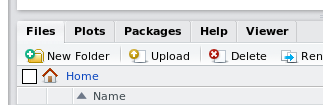
\includegraphics[scale=.5]{RstudioFiles}

The file viewer gives you access to your files.  You should have several files with names like 'lab\_0\_sandbox.Rmd' or 'lab\_4\_thebet.Rmd'.   These files are the R notebooks which your weekly homework assignments.  The files download automatically \textbf{if you directory does not already contain a file with the same name}.  This means that if, while working on one of your assignments, you decide to declare bankruptcy and start over, you can simply delete or rename the file (check the box and hit the delete or rename button) then log out and log back in and a fresh copy of the file will be there.

\item To work on a homework assignment, simply click on the blue hypertext file name

\includegraphics[scale=.5]{RstudioHyplink} and behold:  the \emph{Console} pane will shrink to a little nothing at the bottom of the window and its former place will be filled with an ``R notebook''.

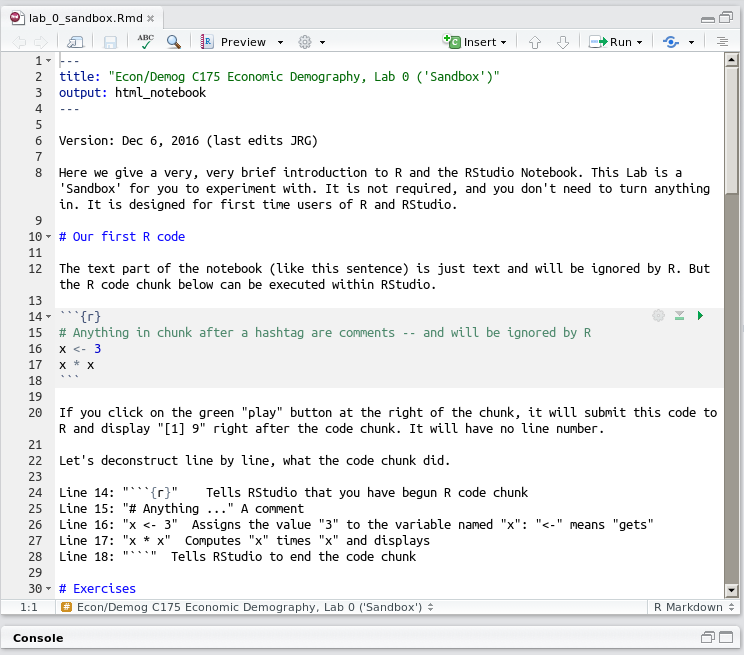
\includegraphics[scale=.3]{RstudioRnotebook}


\end{itemize}

\section{Working in Rstudio}

The majority of your work should be within the ``R notebook''.  That is, most of what you will do for homework will be to read the instructions (in the R notebook); then execute some code; then change the code and execute it again.

The purpose of the code is to learn. Once you have learned what you can from the code, you will go to Bcourses and answer the questions at the end of each R notebook.   

\subsection{Executing code chunks}

In the R notebook, code comes in ``chunks'' interspersed with regular text such as this.  The code chunks look like this:

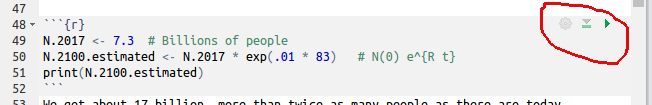
\includegraphics[scale=.5]{RstudioChunk}

They are set off from the text by a light gray background and have three buttons in their upper right corner.  The green triangle on the far right is the most useful, it executes the code \textbf{in the current block only}. You'll generally want to use this button after making changes to the code chunk.

\subsection{Checking your work}

In order to keep you from going off the rails, each R notebook contains a few special code chunks which are designed to check your work. This is not for grading purposes, but rather to let you know that you are doing things right.

The special code chunks look and function the same way other code chunks function-- you make changes to the code then execute it by hitting the green triangle.

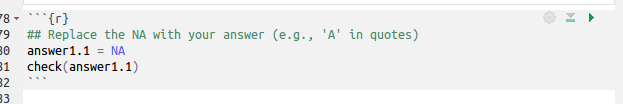
\includegraphics[scale=.5]{RstudioCheck}

The difference is that these code chunks expect you to change only the line that assigns a value to a variable called \textbf{answer1.1} (1.1 will of course change).  After specifying the answer and running the code chunk, you will receive either a dopamine rich message of congratulations, or encouraging hint.  You may execute these chunks as many times as you wish. Their purpose is to help you --not to judge you.

\subsection{Bcourses}

When you have finished the week's R notebook, visit Bcourses and answer the questions pertaining to the assignment that you just did.  The Bcourses part of each week's assignment will be graded.

\section{Resources for learning R, R studio and R notebook}

There are three distinct parts to the learning infrastructure that we will use in Demog/Econ C175: 
\begin{enumerate}
\item \textbf{R} the venerable programming language
\item \textbf{R studio} the new-ish IDE for programming in R
\item \textbf{R notebook} the very new file format for mixing R code and text.
\end{enumerate}


\subsection{R}
\label{sec:R}

Of these three, R, the programming language is by far the hardest. Luckily, there are numerous free web resources to help.
Type ``learn R'' into your favorite search engine for a more comprehensive list list, but here are some favorites of ours:

\begin{enumerate}
\item \url{tryr.codeschool.com}  Great magical browser interface for learning basics of  programming in R. \textbf{the first five chapters are required for this course}

\item
  \url{https://cran.r-project.org/doc/contrib/Torfs+Brauer-Short-R-Intro.pdf}
  \emph{(very) short introduction to R} A fairly complete, and not
  that short, overview of the R language. Note that RStudio has
  changed a lot recently so don't pay too much attention to their
  description of R studio. But otherwise a very good overview,
  especially for those with a bit of computing experience. Even raw
  beginners may find this useful to skim, particularly after having
  tried the first few labs.

\item Google developers youtube videos "Intro to R"
For those who prefer videos, this is a great series. Just note that
they do not use RStudio, so you'll need to modify a few of the
commands. 

\item \url{https://www.datacamp.com/home} Data Camp has videos and exercises. The first course in R is free and quite good.  It takes a bit longer than Codeschool because it is a bit more thorough. 





\end{enumerate}

\subsection{R notebook}
\label{sec:Rnote}

R notebook is quite new, so there are few resources for learning about it. If you have had experience with Jupyter Notebook (as used in Data Science 8) you'll get the idea pretty fast. 
\begin{enumerate}
\item \url{https://www.rstudio.com/resources/webinars/introducing-notebooks-with-r-markdown/} A ``webinar'' produced by rstudio.com.  Its interesting, but you probably don't need it in order to succeed in this class.
\end{enumerate}

\subsection{R studio}
\label{sec:Rstud}

R studio is both new-ish and quite complex. For this course, the key thing is to avoid being distracted by all the shiny objects that R studio presents.  We intend to use just a tiny fraction of the features that R studio makes available.
\begin{enumerate}
\item \url{https://www.rstudio.com/resources/webinars/} rstudio.org has produced several ``webinars'' on Rstudio.  We don't think you \textbf{need} to  use any of them, but if you like this sort of thing...
\end{enumerate}

\section{Piazza}
\label{sec:piazza}

Students are highly encouraged to post their questions (and answers)
on any R programming questions to Piazza. We want this to be a common
resource that will enable you to learn from each other. The graduate
students enrolled in Demog/Econ C175 have kindly agreed to help answer your R
questions. (No question is a bad question. Just remember, "Always be
nice!")

\end{document}

%  LocalWords:  Rstudio edu IDE IDEs Rmd Bcourses
